\documentclass[tikz,border=5pt]{standalone}
\usepackage{tikz}
\usetikzlibrary{matrix,positioning}

\begin{document}
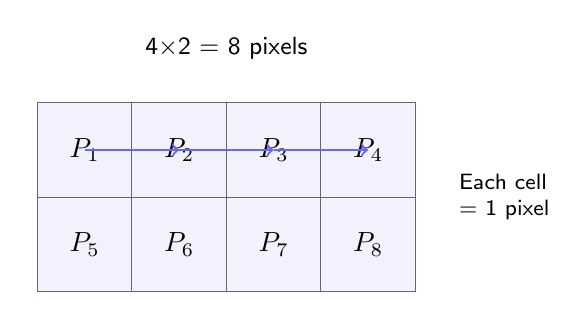
\begin{tikzpicture}[
    cell/.style={minimum width=1.2cm, minimum height=1.2cm, draw=black!60, fill=blue!5},
    label/.style={font=\footnotesize\sffamily}
]

% Pixel grid
\matrix (grid) [matrix of nodes, nodes={cell}, row sep=-\pgflinewidth, column sep=-\pgflinewidth] {
    $P_1$ & $P_2$ & $P_3$ & $P_4$ \\
    $P_5$ & $P_6$ & $P_7$ & $P_8$ \\
};

% Labels
\node[above=0.3cm of grid, font=\sffamily\small] {4$\times$2 = 8 pixels};
\node[right=0.3cm of grid.east, label, align=left] {Each cell\\= 1 pixel};

% Arrow showing scan order
\draw[->, thick, blue!60] (grid-1-1.center) -- (grid-1-2.center);
\draw[->, thick, blue!60] (grid-1-2.center) -- (grid-1-3.center);
\draw[->, thick, blue!60] (grid-1-3.center) -- (grid-1-4.center);

\end{tikzpicture}
\end{document}
